\section{Data, reproduction, and status of the claims}\label{sec:datos}
This section brings together the data accompanying the paper, explains how to repeat the
calculations, and specifies the type of evidence supporting each claim.

\subsection{Comparison with the exact counts}
For the sizes studied, $Q(n)$ is known exactly~\cite{oeis,q27}.
Figure~\ref{fig:counts} shows $nR_Q(n)$ for $16\le n\le27$, calculated by taking the logarithm of
the integer count and subtracting, before multiplying by $n$, the numerical logarithm of the
predictor. A period-four oscillation is observed at these twelve sizes. A fit with $\cerr$ fixed in
advance and a correction $a/n$ describes part of the variation (Appendix~\ref{app:numquad}).
These data are consistent with the estimate of $\cerr$. The counts and the values of the predictor
are in \texttt{suplemento/datos/c\_n.json}.
\begin{figure}[ht]
\centering
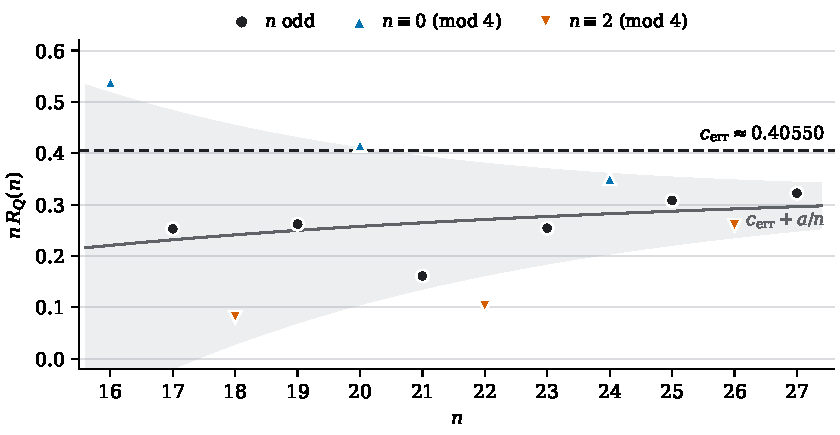
\includegraphics[width=.9\linewidth]{figuras/conteos.pdf}
\caption{Values of $nR_Q(n)$ for $16\le n\le27$, obtained from the exact counts and the canonical
predictor (numerical evidence). The dashed line marks the estimate of $\cerr$. The gray curve shows
the fitted drift $\cerr+a/n$, with $a\simeq-2.956$, and the shaded band has the amplitude
$Ae^{-\kappa(n-16)}$ of the period-four oscillation (Appendix~\ref{app:numquad}). The odd sizes lie
near the drift. Multiples of four lie above it, and those that leave remainder two when divided by
four lie below it.}\label{fig:counts}
\end{figure}


\subsection{Reproduction of the numerical value}
The supplement contains the final grids, the analysis programs, the values at the nodes, the
intervals, and the SHA256 hashes of all the files.
With Python~3 and NumPy, the command \texttt{python -B replica/reproducir\_valor.py replay}, run
from \texttt{suplemento}, repeats the analysis in a new directory and should give $0.4055003786$ to
ten decimal places. The guide in the supplement also explains how to regenerate the grids from
scratch. The main run comprised 955 tasks and took 168.3 minutes with 16 processes; the
supplementary run comprised 132 tasks and took 30.1 minutes.

\subsection{Interval certificates}
In \texttt{suplemento/certificados} are the programs that generate the intervals for the profile,
for $S$, for $P_T$, and for $Q_2$ at the tenth node of the twenty-point Gauss--Legendre rule,
together with the signed bivariate kernel at that node and a quick test of the inputs. Each
certificate records the precision used, its inputs, and the interval obtained;
Section~\ref{sec:numcert} explains what is certified and to what extent.

\subsection{Registered predictions}
In the finite-board checks, the prediction, the cases, and the comparison rule were fixed before
evaluation in a file with a timestamp and a SHA256 hash. The square study, for example, registered
eleven predictions: eight in blind cases and three in known controls.
